\section{House Model Machine Learning}

\subsection{Introduction}\label{s:introduction}
The developed house model [\url{https://hancse@github.com/hancse/twozone\_housemodel.git}] allows to simulate the heat demand of a given house. Based on weather information such as the outside temperature and solar irradiation, house specifications, and other input factors it is possible to compute the details of the temperature evolution. 

The model needs many details to run. These details will be hard to get a hold of in practice.

It would be interesting to see whether it is possible to use machine learning to abstract from the details that are used to create the model and use only limited amount of input data to create a model that can predict the heat demand of a house. 

 


%\section{Background}\label{s:background}


\subsection{Machine learning approach}\label{s:MLA}


\subsubsection{LSTM network}
We create a Long Short-Term Memory (LSTM) network for predicting the heat demand. An LSTM network is a type of recurrent neural network (RNN). These models are widely used in, for example, the field of speech recognition, language modeling, and machine translation. LSTM networks are also well suited for time series data, as we have here. In a RNN the output of a layer in the network can be fed back to be used as input of an earlier layer in the network. In this way, dependencies on the data history can be taken into account in the model. LSTM networks are a specific type of RNNs, designed such that the network learns which historical data is needed to 
"remember" using the memory cell, and which data can be "forgotten" using a so-termed forget-gate, in order to predict the next output. More background on the working of the LSTM can be found in \cite{LSTM}, a blog by Christopher Olah with a comprehensive explanation of the ideas behind the LSTM network. 

The full network that will be used consists of an LSTM-layer, that is used to learn the dependencies on the historic data, and a fully connected linear layer that applies a linear transformation to the output from the LSTM-layer to obtain the final output, the predicted heat demand. 



\subsubsection{input data selection}

In this first exploration of the potential of using a machine learning model to predict the heat demand of a household we make use of data generated with the house model. The house model can provide a heat demand profile for a full year. The heat demand is based on weather data, temperature and solar irradiation, construction parameters of the house, and some behavioral parameters, such as the number of people present in the house and the thermostat setting.   

The model is described in detail in [ref to document of the house model]. The house is modeled as a network of thermal capacitors, between which energy can be exchanged. The most simple house model uses 2 thermal capacitors, one for the air in the house and one for the walls. Heat can be exchanged between the two capacitors, and the outside air. Essentially this model approximates the house as a single compartment with its walls. 

A more detailed representation of the house can be made by using multiple heat capacitors, for example one for each floor or room.   
Several versions of the specific model have been developed. A first version is created in Matlab-Simulink, and a more elaborate version is under development using Python. 

Initially, we have made use of the data generated by the Matlab-Simulink implementation, which has a time granularity of one hour. Later we have shifted to the more detailed Python implementation of the model, which has more flexibility and a finer time granularity.

The input features we want to use for our model are the same for both the Matlab-Simulink model and the Python model. These should also be easily available in practice. The input features we select to create our model are:
\begin{itemize}
\item Outside temperature ($T_{out}$); we can assume this parameter is easily available through either a local thermometer or an online service providing data of a nearby weather station. Alternatively weather forecast date might be used. 
\item temperature of the house ($T_{house}$); this should be available through the thermostat. In the house model this is the temperature of air. In case of a model that has multiple compartments, we use the air temperature of the main compartment.
\item thermostat set point ($SP$), this should be available though the thermostat. Potentially, these values are even available for future values, since often programs are created to set the thermostat values. 
\item solar irradiation ($Q_{solar}$), although these values may not be straightforward to obtain for a specific location, an estimate value may be obtained from a local weather station. 
\item heat demand ($Q_{demand}$), the historic values of the heat demand will be used to predict the future values. 
\end{itemize}

More features could be available from the house model, such as the heat generated by the appliances and inhabitants or the temperature of the walls. However, not all of these will be practically available. We hope to obtain a machine learned model that can abstract from these details and still give a good prediction for the heat demand for the coming time period. When much data from the house model is needed that is not measured in practice, it is unrealistic the machine learned model could be transferred to a scenario where it works with real life data.  

\textit{NOTE: It might be interesting to also look at the capabilities to predict the house temperature as well. For the other inputs a future value may be obtained from either the weather forecast or the thermostat program. Taking the temperature predictions into account might be helpful for a model predictive control approach?}

\subsubsection{data preprocessing steps}
The input data is loaded from an Excel sheet that contains all the hourly values. When we want to create a model the data needs to be split in a training and a test set. As we are dealing with a time series the order of the data needs to be retained. The first $70\%$ of the data will be used for training the mode and the last $30\%$ will be used for testing. 

Next to splitting the data, the data set needs to be normalized, by subtracting the mean of all feature values ($\mu$) and dividing by the standard deviation ($\sigma$) (using the \texttt{standardscaler}),$x_{norm}= \frac{x-\mu}{\sigma}$. The output is normalized as well.

After the normalization of the data, the data needs to be prepared for the LSTM. From the data a set of sequences is created. For each output value, heat demand at time $t$, a sequence of historical data of input values is needed, time steps $t-N \cdots t-1$.  

\textit{NOTE: the value of N, the number of historical time steps needs to be determined. For the hourly data $N=12$ seems to give good results. A logical choice would be to set $N$ such that 24 hours of historical data is used to predict the next time step, since a high correlation with 24 hours earlier is to be expected. The actual number of time steps depends on the time granularity of the data. 
One may also reason that the heat demand for the next hour is mainly determined by the temperatures and the thermostat setting of the last hour. This implies little history is actually needed.} 

\subsubsection{model training}
In order to train the network, we pass all input data through the network. The mean squared error of the result is computed, and using the Adam-optimizer algorithm the network is improved. The Adam-optimizer is currently one of the most used algorithms, and in many cases gives a faster convergence (check the reference given on https://machinelearningmastery.com/adam-optimization-algorithm-for-deep-learning/). However, it may be useful to investigate the performance of other optimizers.
 
The steps of passing the data through the network and further optimization are repeated for several iterations, or epochs.
 
%
%\begin{itemize}
%\item What are the options for settings for the learning process?
%\item Adam learning algorithm
%\item number of epochs
%\item \ldots
%\end{itemize}
%


\subsubsection{model testing}
After the network has been trained, the obtained model is tested with the test data. The test data consists of the last 30\% of the data sequence obtained from the house model. This data needs to be preprocessed in the same way as the training data. So, we need to scale the data and create the input sequences that are used to predict the next output. 

The output obtained form the network, needs to be scaled back so it can be compared with the real values that have been obtained from the house model. As error metric, we use the RMSE (Root mean squared error). 

\subsubsection{model optimization}
The LSTM network contains several parameters that can be adapted to optimize the learning process, and the quality of the final model.The key parameters are:
\begin{itemize}
\item number of hidden neurons or number of output neurons of the LSTM layer: By increasing this parameter the network complexity is increased. A more complex allows for closer fitting to the training data. However too many hidden neurons may result in an overfitted model. 
\item sequence length: By increasing the sequence length the model takes a larger portion of the history into account for the prediction of the next value. This comes at the cost of a longer computation time. 
\item number of optimization iterations (epochs): By optimizing over more iterations the algorithm has a higher chance to find the optimal model configuration. This comes at the cost of a longer computation time. In general you will see that the gain of model quality is highest in the start of the optimization process. The trade off between increased model accuracy and additional computation time worsens when the number of iterations is large. 
\item learning rate: The learning rate influences the step size that will be taken in the optimization process. This is a parameter that is used by the Adam optimization algorithm. 
\end{itemize}


%\section{Python implementation}
 %various functions
%
%\subsection{LSTM-layer}
%The key parameters that need to be defined for the LSTM-layer are:
%\begin{itemize}
%\item input\_size: the number of input features used for the layer.
%\item hidden\_size: the number of features in the hidden state.
%\end{itemize}
%All other parameters, such as, num\_layers, bias, etc, will be used in the default setting. 
%




\subsection{results}
In this section we look at the first results obtained with the neural network for both the data obtained with the Matlab-Simulink model and the Python model. 



\subsubsection{Matlab-Simulink housemodel}
In this analysis we have trained the model on the data from the Matlab-Simulink model for a light weight construction.  
At the moment of writing this document the specifics on the used input to create the data set are unknown to the author. 

The dataset contains hourly values for the features:
\begin{itemize}
\item temperature\_house: the temperature of the air in the house (in degrees centigrade). 
\item heat\_demand: average power demand to heat the house (in W)
\item setpoint\_temperature: thermostat setpoint (in degrees centigrade)
\item temperature\_outside: the outdoor temperature (in degrees centigrade)
\item heat\_solar: the heat added to the house by the sun (in W), based on the NEN-5060 \cite{NEN5060}. 
\item temperature\_wall: temperature of the walls (in degrees centigrade)
\item heat\_internals: estimate for heat from people and devices present in the house (in W) 
\end{itemize}

From this set we use only the features, temperature\_house, setpoint\_temperature, temperature\_outside, heat\_solar and heat\_demand. 
The LSTM-layer in the network has 20 output nodes, and we use a learning rate of 0.01. Some experimenting shows that after 1000 training epochs little further improvement is made. The obtained model will predict only the next value, i.e., the average heat demand for the next hour, based on the input. 

We vary the input sequence length to see how much history we need to take into account in the training of the model. The results are summarized in Table \ref{tab:results_simulink}. The table shows both the training loss and the test RMSE for various values of the sequence length. The training loss is the MSE of the model on the normalized training data. The RMSE for the test data is based on the real non-normalized heat demand values. \textit{(NOTE: For comparing training and test, it is needed to evaluate them both on the real values.)}

In Table~\ref{tab:results_simulink}, we can see that the best results are obtained for the sequence length of 18. It is likely that the shorter sequence lengths have worse results due to a lack of historical information. For the models with longer sequences the performance might get worse due to the higher model complexity. This implies that training over more iterations is needed to achieve the same level of accuracy. It is also important to note that when the sequence length is increased, the computation time for every iteration in the optimization process is increased as well.
  
\begin{table}[H]
	\centering
		\begin{tabular}{c|c|c}
			\hline
			seq length & train loss & test RMSE  \\
			\hline
			\hline
			2 & 0.256 & 1529\\
			4 & 0.135 & 1562\\
			8 & 0.083	& 681\\
			12 & 0.015 & 316\\	
			16 & 0.014 & 291\\
			18 & 0.011 & 275\\
			24 & 0.010 & 293\\
			32 & 0.013 & 336\\
			\hline
		\end{tabular}
	\caption{training loss and test MSE for varying values of the sequence length}
	\label{tab:results_simulink}
\end{table}


\begin{figure}[H]
	\centering
		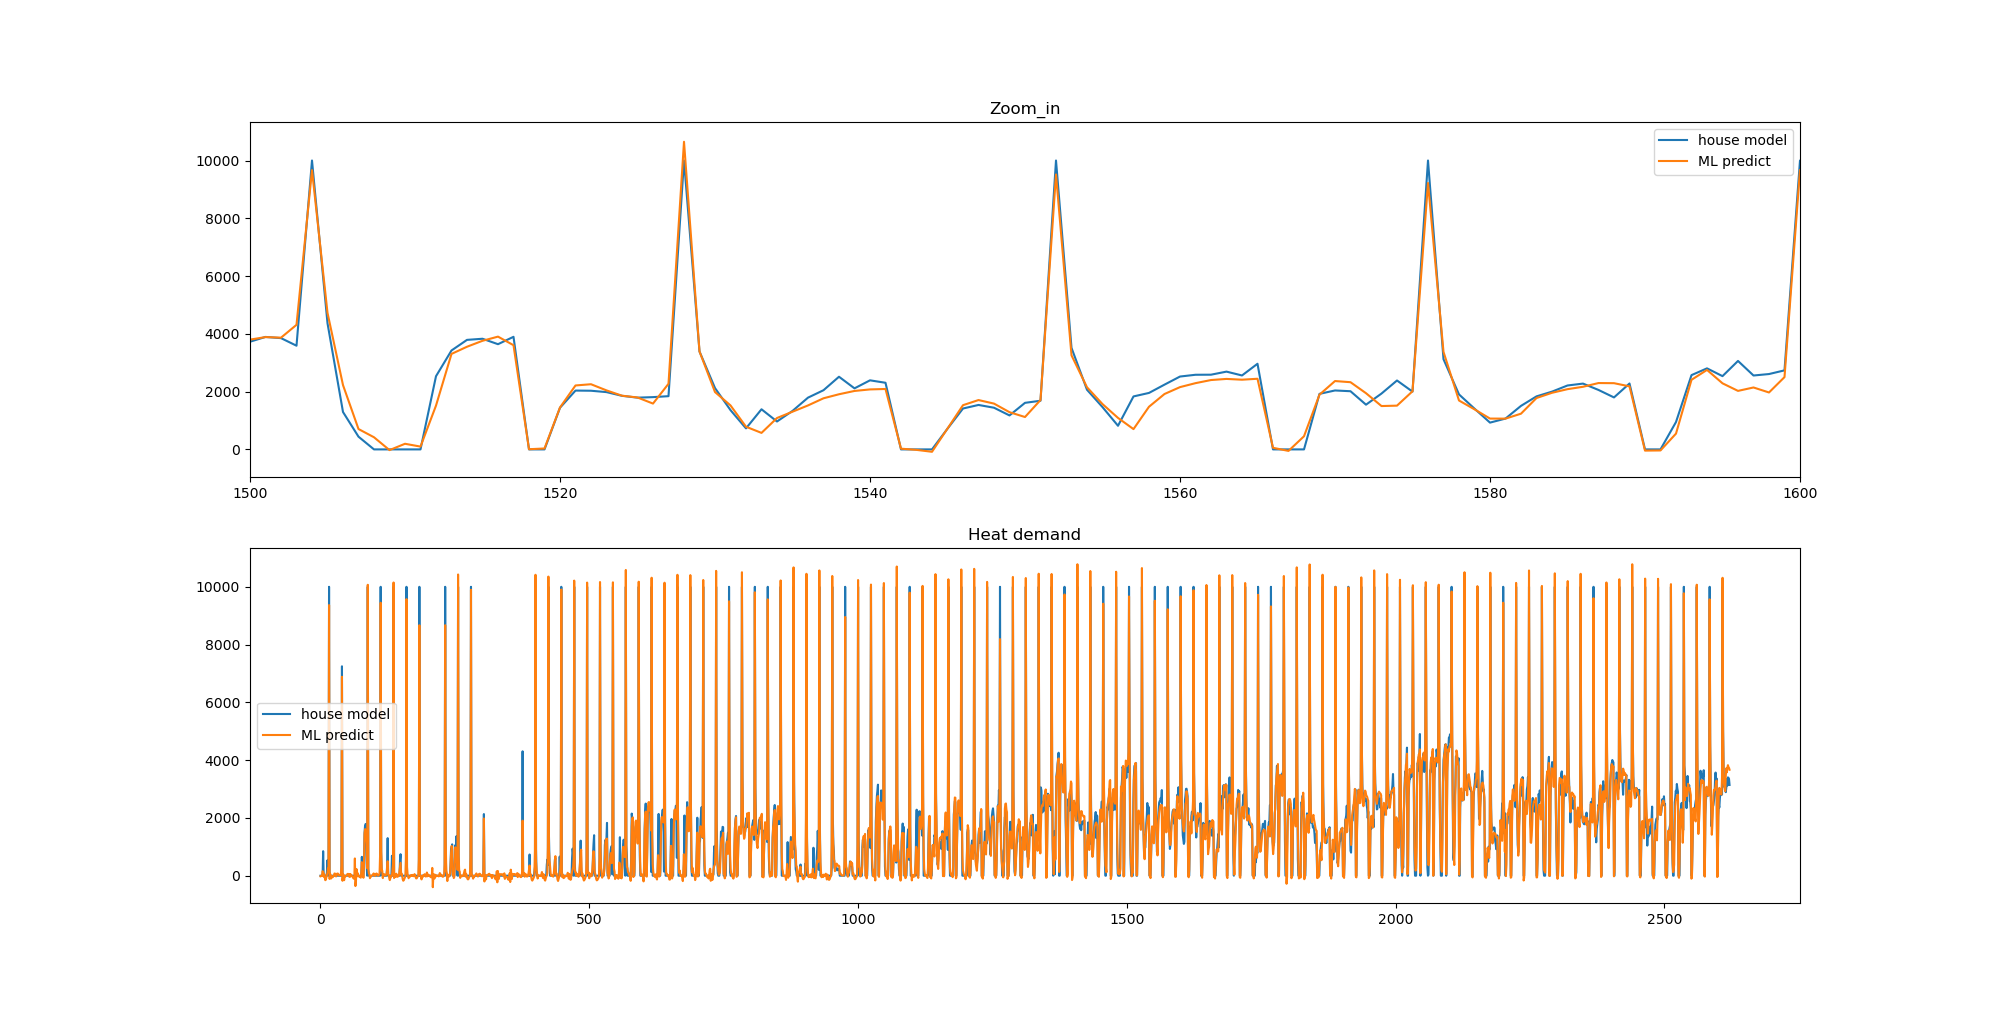
\includegraphics[width = 0.9\textwidth]{figures/seq_18_epoch_1000_Matlab1.png}
		\caption{heat demand for Matlab Simulink model and the ML predictions.}
	\label{fig:matlab_seq18}
\end{figure}

Figure~\ref{fig:matlab_seq18} shows the heat demand according to the Matlab-Simulink model and the ML-predictions when using a sequence length of 18 samples. The figure gives the results for the test set, that is the last 30\% of the year. The x-axis is labeled with the index of the array (corresponding to number of hours after the start), the y-axis is the average heat demand in the hour in W. 

We see that the ML-model matches the general trend of the Matlab-Simulink model. The RMSE of the ML-prediction is 275~W, while the average value is roughly 3000~W. 


\subsubsection{Python house model}
In this analysis we train the data on the Python house model. The data is generated with the version \texttt{Simulation\_for\_companies.py}. This model has a time granularity of 10 minutes, thus 6 values per hour. An excel-file, \texttt{tst\_ML.xlxs}, with output data from the model is generated. The same features as for the Matlab-Simulink model are used: House temperature, thermostat setpoint, outside temperature, solar irradiation and heat demand. Note that, here the solar irradiation is derived from the NEN-5060 global irradiation values \cite{NEN5060}. By interpolation the hourly values from the NEN-5060 are converted to values for every 10 minutes.  

Due to the finer time granularity the ML learning process takes much longer than for the Matlab-Simulink based dataset. First of all, the data set is ten times larger. Furthermore, a larger number of datapoints needs to be used to build the same time span of historical values. Both have a big impact on the computation time. Where the Matlab-Simulink data is trained in a couple of minutes, the Python data takes hours to process on my laptop. 

Furthermore, the model still predicts only for the next time instance. Thus, in for the Python data a prediction for the next 10 minutes interval is made.  

Some explorative experiments have been performed for which the results are summarized in Table \ref{tab:results_python}. Note that the RMSE values are a factor 1000 lower than for the Simulink model. This is due to the fact that the Python model outputs the heat demand in kW instead of W. 

\begin{table}[H]
	\centering
		\begin{tabular}{c|c|c|c}
				\hline
					seq length & nr epochs & train loss & test RMSE  \\
				\hline
				\hline
					24 & 700 & 0.0278 & 0.363 \\
					36 & 1000 & 0.0209	& 0.349 \\
					72 & 700 & 0.0258	& 0.352 \\
					84 & 1000 & 0.0183 & 0.301\\
					144 & 50 & 0.0601 & 0.525\\
					\hline
		\end{tabular}
	\caption{training loss and test RMSE for varying values of the sequence length and number of epochs. }
	\label{tab:results_python}
\end{table}
 

\begin{figure}[H]
	\centering
		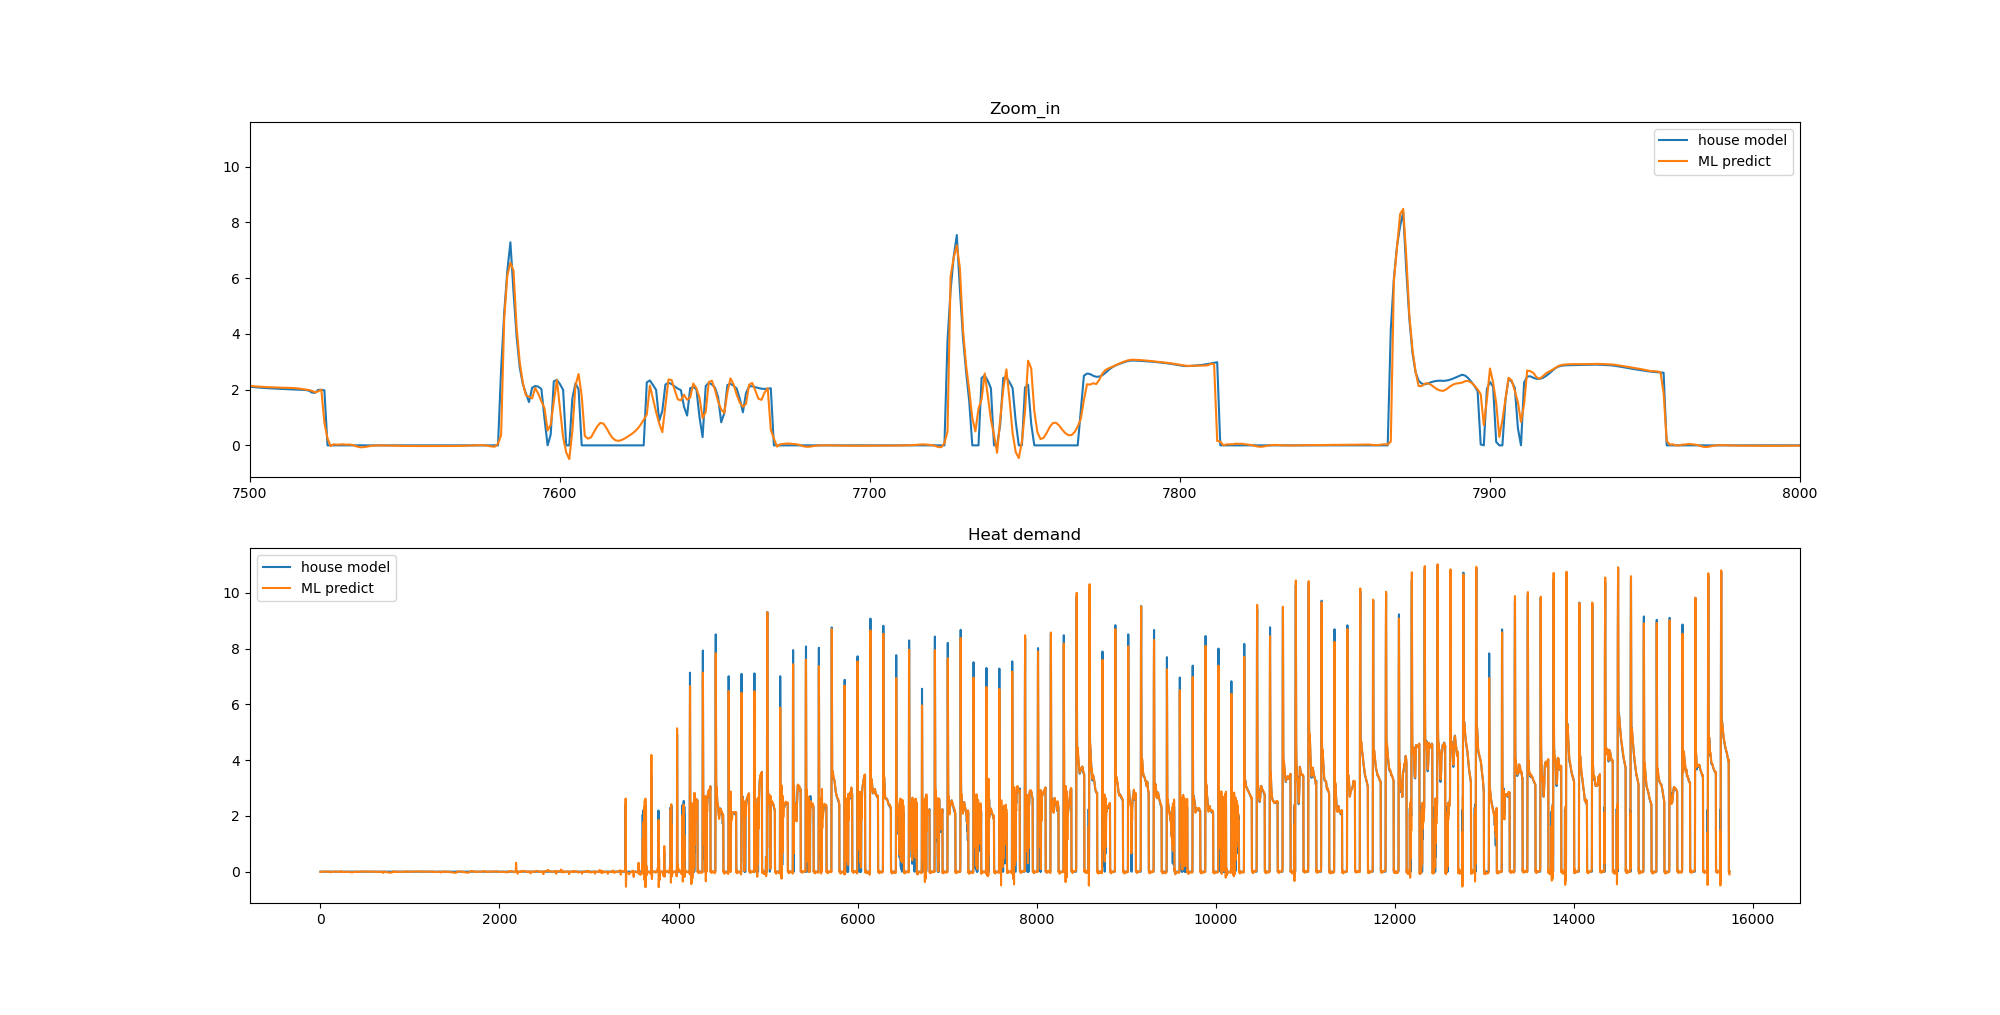
\includegraphics[width = 0.9\textwidth]{figures/seq_84_epoch_1000_Python1.png}
		\caption{heat demand for Matlab Simulink model and the ML predictions.}
	\label{fig:python_seq84}
\end{figure}

In figure \ref{fig:python_seq84} we see the plot of the heat demand according to the Python model and the predictions from the ML-model. Again, the prediction matches the general trend well. However, due to the smaller time granularity, the heat demands contains more variation during the day. This behavior is harder to learn for the ML-model. In some cases the ML-model seems to trail the original data with one time step. Further investigation is needed to see whether the ML-model in these cases mainly reacts on the last value of the heat demand or not. In addition it would be interesting to see whether it is possible to predict the heat demand for a larger time span than only 10 minutes. 

\subsection{conclusion}
The LSTM-network has potential to learn a model that mimics the behavior of the Python house model. However, further research is needed after the initial investigations to get more insight in what the model really can do. Training for over more epochs and with longer historic sequences could give better results.  Also further optimization over the different model parameters is possible. 

Next to optimizing the training process, it would be interesting to further investigate the possibility to predict over a longer time span. Furthermore, it would be interesting to see generic the model is, by looking at predictions for other house configurations. A more general model might be also possible to obtain by training over a wider spectrum of house configurations from the python program. 

Other questions that pop-up:
\begin{itemize}
\item Is it possible to reduce the input, for example can we predict the heat demand without using the history as input?
\item Is it possible to predict the indoor temperature as well? This might be useful for making predictions over a longer time horizon. (weather forecasts and the thermostat program can be used for the other features in the prediction)  
\item Is it possible to use the prediction from the ML model for a model predictive control approach?
\item Would the methodology work on real data from a house? 
\item How much data is needed to train the model sufficiently? Would it be possible to create a "compressed year" with the essential variations on which the model can be trained faster? 
\end{itemize}


\subsection{Python files}
The python files for doing the machine learning are located in the repository, in the directory \texttt{ML\_heat\_demand}. 

\texttt{test\_example.py} will run the machine learning process. Inside this function parameters, like the number of epochs, the number of hidden neurons and the sequence length, can be changed. 

\texttt{load\_and\_preprocess\_training.py} contains the functions that are used for loading and preprocessing the data. 

\texttt{LSTM\_model\_struct.py} builds the LSTM-network, consisting of a LSTM-layer and a fully connect linear layer. 

\texttt{train\_model.py} trains the network on the training data. 

\texttt{Prediction.py} computes the prediction for the test data set. 

The directory \texttt{data} contains the excel input files that were used to create the results in this document, \texttt{test\_excel.xlsx} for the Matlab-Simulink data and \texttt{tst\_ML.xlsx} for the Python model data. Also, the obtained model is saved here as \texttt{test\_model}.

